\documentclass[tikz,convert={outfile=monoid-in-moncat-unitality.svg}]{standalone}
\begin{document}
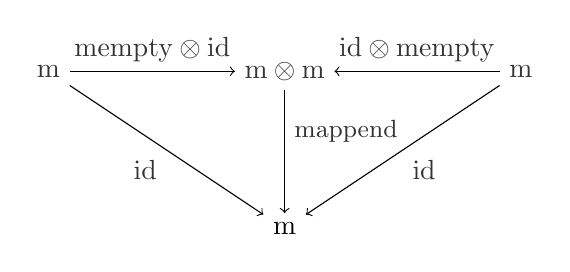
\begin{tikzpicture}
    \node (A) at (0,2) {\textcolor{black!80}{\(\mathrm{m}\)}};
    \node (B) at (3,2) {\textcolor{black!80}{\(\mathrm{m\otimes m}\)}};
    \node (C) at (6,2) {\textcolor{black!80}{\(\mathrm{m}\)}};
    \node (D) at (3,0) {\(\mathrm{m}\)};
    \draw [->] (A) -- node[above] {\textcolor{black!80}{\(\mathrm{mempty\otimes
    id}\)}} (B); 
    \draw [->] (C) -- node[above] {\textcolor{black!80}{\(\mathrm{id\otimes
    mempty}\)}} (B);
    \draw [->] (B) -- node[above right] {\textcolor{black!80}{\small\(\mathrm{mappend}\)}}  (D);
    \draw [->] (A) -- node[below left]  {\textcolor{black!80}{\(\mathrm{id}\)}} (D);
    \draw [->] (C) -- node[below right] {\textcolor{black!80}{\(\mathrm{id}\)}} (D);
\end{tikzpicture}
\end{document}
